\documentclass[10pt,a4paper]{article}

% ---------- Codificación e idioma ----------
\usepackage[utf8]{inputenc}
\usepackage[T1]{fontenc}            % acentos y guiones bien en el PDF
\usepackage[english]{babel}
\DeclareUnicodeCharacter{2212}{-} % el signo menos Unicode no rompe la compilación

% ---------- Página ----------
\usepackage[a4paper,margin=2cm]{geometry}   % 2 cm: límite de 2 páginas
\usepackage{microtype}              % mejor reparto de espacios, ahorra líneas
\usepackage{multicol}

% ---------- Matemáticas ----------
\usepackage{amsmath,amssymb,amsthm}

% ---------- Unidades y química ----------
\usepackage{siunitx}
\sisetup{per-mode=symbol}           % kcal/mol en vez de kcal mol^-1
\DeclareSIUnit\calorie{cal}         % ¡usar \kilo\calorie, no \kilo\cal!
\DeclareSIUnit\atm{atm}
\DeclareSIUnit\hartree{\ensuremath{E_\mathrm{h}}}
\usepackage[version=4]{mhchem}

% ---------- Figuras y tablas ----------
\usepackage{graphicx}
\usepackage{booktabs}
\usepackage{float}
\usepackage[font=small,labelfont=bf]{caption}
\usepackage{tikz}
\usepackage{pgfplots}
\pgfplotsset{compat=1.18}
\renewcommand{\topfraction}{0.92}
\renewcommand{\textfraction}{0.05}

% ---------- Otros ----------
\usepackage[normalem]{ulem}         % normalem: \emph sigue siendo cursiva

% ---------- Compactación (para el límite de 2 páginas) ----------
\usepackage{titling}                % título más compacto
\setlength{\droptitle}{-1.6cm}
\pretitle{\begin{center}\large\bfseries}\posttitle{\par\end{center}\vspace{-0.6em}}
\preauthor{\begin{center}\normalsize}\postauthor{\par\end{center}\vspace{-0.9em}}
\predate{\begin{center}\small}\postdate{\par\end{center}\vspace{-1.2em}}
\usepackage{titlesec}               % secciones con menos espacio alrededor
\titleformat{\section}{\large\bfseries}{\thesection}{0.6em}{}
\titlespacing*{\section}{0pt}{1.1ex plus 0.3ex}{0.5ex}
\usepackage[shortlabels]{enumitem}  % listas sin espacios extra
\setlist{nosep, leftmargin=*}
\setlength{\intextsep}{6pt plus 2pt minus 2pt}       % espacio alrededor de figuras/tablas [H]
\captionsetup{skip=4pt}
\setlength{\parskip}{0pt}
\usepackage{etoolbox}               % bibliografía más pequeña y sin huecos
\apptocmd{\thebibliography}{\footnotesize\setlength{\itemsep}{0pt}\setlength{\parsep}{0pt}}{}{}

% ---------- Referencias (siempre al final y en este orden) ----------
\usepackage[hidelinks]{hyperref}
\usepackage[capitalise,noabbrev]{cleveref}



\title{One molecule versus many copies:\\ubiquitin flexibility from 100 ps of MD against crystallographic B factors}
\author{Martín Llorens Giménez\thanks{\textbf{Declaration of AI use:} Claude Opus 5.5 (Anthropic) to assist with VMD, awk, and NAMD command syntax, generate Python plotting scripts, and for translation, language editing, and improving the readability of the manuscript. All simulations, data analyses, and numerical results were independently performed and verified by the author.}}
\date{November 2026}


\begin{document}

\maketitle

\section{Introduction}
Ubiquitin is a small (76 residues), highly stable protein with a compact $\beta$-grasp fold and a flexible C-terminal tail, and a high-resolution crystal structure is available (PDB 1UBQ~\cite{1ubq}), which makes it a standard test system for molecular dynamics (MD). In this work, a \SI{100}{ps} MD trajectory of ubiquitin in water is analysed for equilibration (energy, temperature and RMSD) and per-residue flexibility. The flexibility obtained from the simulation is then compared, residue by residue, with the crystallographic temperature factors of the structure the simulation started from, in order to separate two questions: whether a short simulation identifies \emph{where} the protein is flexible, and whether it reproduces \emph{how much}.


\section{Methods}

A \SI{100}{ps} molecular dynamics trajectory of ubiquitin (76 residues) in explicit water, provided with the practical session, was analysed. It was generated with NAMD~\cite{namd} using the CHARMM27 force field with CMAP corrections~\cite{charmm22,cmap} and the TIP3P water model~\cite{tip3p}, in an orthorhombic periodic box of $38.7\times40.5\times\SI{43.3}{\angstrom}$ containing 7051 atoms. The production run was carried out in the NVT ensemble with a Langevin thermostat~\cite{bbk} at \SI{300}{K} ($\gamma = \SI{10}{ps^{-1}}$), a time step of \SI{1}{fs} with all bonds flexible, and non-bonded interactions smoothly switched off between 10 and \SI{12}{\angstrom}, without Ewald summation. It was preceded by \SI{50.5}{ps} of equilibration. The starting structure derives from the crystal structure 1UBQ~\cite{1ubq}: without any superposition, its C$_\alpha$ atoms deviate from those of 1UBQ by an RMSD of \SI{1.06}{\angstrom} (maximum \SI{1.99}{\angstrom}, Gly10).

Trajectories were analysed with VMD~\cite{vmd} (400 frames, one every \SI{0.25}{ps}). Running averages of the energy and temperature were computed from the NAMD log, which only reports averages over each output interval. The heavy-atom RMSD of the protein was computed after least-squares fitting to the starting structure. For the root-mean-square fluctuation (RMSF), every frame was fitted on the C$_\alpha$ atoms of residues 1--70, excluding the C-terminal tail so that its large motion does not bias the superposition, and the RMSF of each C$_\alpha$ was computed over the structurally equilibrated window (32--100\,ps). It was converted into an isotropic temperature factor, $B_\mathrm{MD} = \tfrac{8\pi^2}{3}\,\mathrm{RMSF}^2$~\cite{hunenberger}, and compared with the C$_\alpha$ $B$ factors of 1UBQ. Secondary structure was assigned with STRIDE~\cite{stride} as implemented in VMD.

\section{Results and discussion}
\label{sec:results}

\textbf{Two equilibration timescales.} The initial velocities correspond to \SI{211}{K}; the thermostat brings the system to \SI{300}{K}, and the total energy to its plateau, in less than \SI{1}{ps} (Fig.~\ref{fig:time}a,b). The protein structure relaxes far more slowly: the RMSD rises for about \SI{30}{ps} before levelling off at \SI{0.95(7)}{\angstrom} (Fig.~\ref{fig:time}c), a value below \SI{1}{\angstrom} that reflects the rigidity of the ubiquitin fold. Block averages show a renewed rise to \SI{1.09}{\angstrom} in the last \SI{10}{ps}; whether this marks the onset of a conformational change cannot be decided within \SI{100}{ps}. Thermal equilibrium is thus reached about 30 times faster than structural equilibrium, and only the latter justifies the averaging window used for the RMSF.


\begin{figure}[H]
\centering
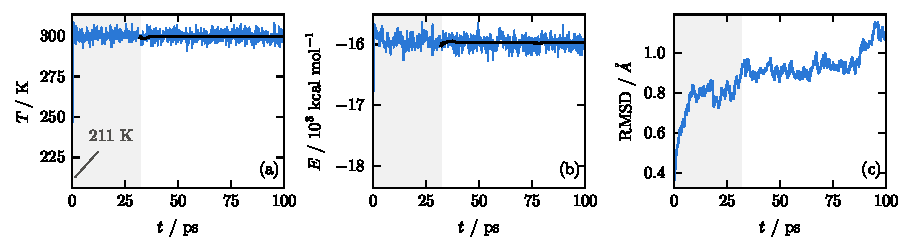
\includegraphics[width=\textwidth]{fig1_ubq_tiempo.pdf}
\caption{(a) Temperature, (b) total energy and (c) heavy-atom RMSD of the protein, relative to the starting structure, along the production run. Black: running averages over the plateau. Shaded: structural equilibration (0--32\,ps).}
\label{fig:time}
\end{figure}

\textbf{Temperature fluctuations.} Over the plateau, $T = \SI{299.9(27)}{K}$. Its relative fluctuation, $\sigma_T/\langle T\rangle = \SI{0.89(1)}{\percent}$ (block averaging), lies \SI{8}{\percent} below the canonical prediction $\sqrt{2/N_\mathrm{df}} = \SI{0.97}{\percent}$~\cite{allen}, whereas the pure-water simulation of this session, run with the same time step and thermostat, reproduces it (\SI{1.41(3)}{\percent} vs.\ \SI{1.41}{\percent}). A counting error is excluded, since $N_\mathrm{df} = 2\langle K\rangle/(k_\mathrm{B}\langle T\rangle) = 3N$ is recovered from the log. As kinetic-energy fluctuations in the canonical ensemble are independent of the potential, the deviation can only arise from how the discretised Langevin dynamics samples this particular system, not from the force field itself; repeating the run with $\Delta t = \SI{0.5}{fs}$ or with constrained X--H bonds would locate it. Its origin remains unidentified.

\begin{figure}[H]
\centering
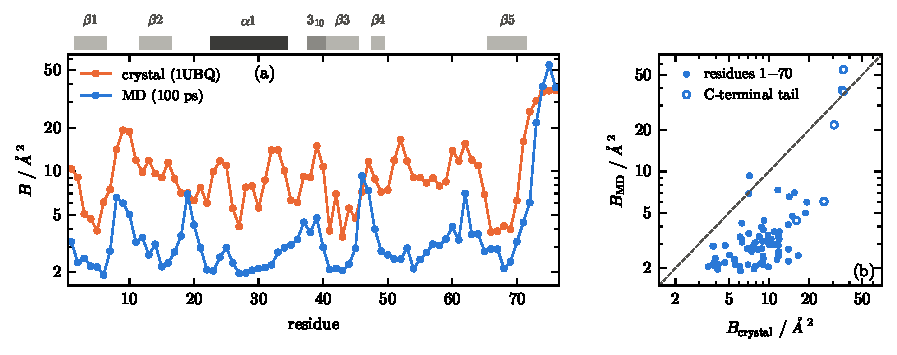
\includegraphics[width=\textwidth]{fig2_ubq_bfactors.pdf}
\caption{(a) C$_\alpha$ temperature factors from the crystal (1UBQ) and from the MD RMSF, on a logarithmic scale, where a constant scale factor becomes a vertical shift; the bar marks the secondary structure. (b) $B_\mathrm{MD}$ against $B_\mathrm{cryst}$; dashed: $B_\mathrm{MD} = B_\mathrm{cryst}$; open symbols: C-terminal tail (71--76).}
\label{fig:bfac}
\end{figure}

\textbf{Flexibility: simulation against crystal.} Both profiles agree on the dominant feature: the C-terminal tail (71--76) is by far the most flexible region, with $B$ of 30--\SI{50}{\angstrom^2} in both (Fig.~\ref{fig:bfac}). At residues 74--75 the simulation even exceeds the crystal (54 vs.\ \SI{36}{\angstrom^2}), plausibly because lattice contacts restrain the tail in the crystal but not in solution. In the core (1--70), however, $B_\mathrm{MD}$ falls short of $B_\mathrm{cryst}$ by a factor of 2.8 on average, as expected: \SI{70}{ps} only samples fast local motions, while crystallographic $B$ factors also contain static disorder and lattice vibrations~\cite{hunenberger}. The location of flexibility is reproduced only partially: the $\beta1$--$\beta2$ loop (7--10) and the region 62--64 appear in both profiles, but the largest core peak of the simulation (46--47) is moderate in the crystal, and crystal maxima such as 34--35 or 52 are absent from the simulation. Over all 76 residues the Pearson coefficient is $r = 0.82$, but it is dominated by the six tail residues (Fig.~\ref{fig:bfac}b); within the core, $r = 0.39$ and the rank correlation is $\rho = 0.43$, a weak-to-moderate agreement.

\section{Conclusion}
The ubiquitin trajectory is thermally equilibrated within \SI{1}{ps} but needs about \SI{30}{ps} to relax structurally, which sets the window for any structural average. Against the crystal, \SI{100}{ps} of MD capture the dominant flexibility of the C-terminal tail and some loops, but underestimate the core by a factor of $\sim$3 and miss the finer ranking of flexible regions; a single global correlation coefficient, set by a handful of extreme residues, would hide this limitation. The temperature fluctuations, 8\,\% below canonical theory while the water control agrees, point to a system-specific sampling artefact that a shorter time step or constrained X--H bonds would test.
{\footnotesize
\begin{multicols}{2}
\bibliographystyle{unsrt}
\bibliography{bibliografia}
\end{multicols}
}

\end{document}
